\chapter{Related Works}
\label{chapter:related}

%\minitoc
\chapterwithfigures{\nameref*{chapter:related}}
\chapterwithtables{\nameref*{chapter:related}}

\ifthenelse{\boolean{skipRelated}}{\endinput}{}

\section{Deep Learning for Computer Vision}

\ac{CNN} have been for a long-time the \textit{defacto} method for \acs{NN} for \ac{CV}
\citep{fukushima1980neocognitron,lecun1999lenet}. In 2012, with larger datasets and better hardware
(\ie \acs{GPU}), \cite{krizhevsky2012alexnet} imposed \ac{DL} models as the best performing
algorithms for images. In the 2010's decade, multiple major improvements were made but the one of
the latest best performing models \citep{tan2019efficientnet} is mainly based on two architectural changes:
residual connections allowing training of very deep networks \citep{he2016resnet} and normalization
of intermediate activations \citep{ioffe2015batchnorm}. Another major factor of recent \ac{CNN}
improvements is better training procedure \citep{wightman2019resnetstrikesback}, which includes
optimizer \citep{kingma2014adam}, learning rate scheduling, strong data augmentations
\citep{muller2021trivialaugment,hingyi2018mixup,zhong2017erasing}, and regularizations
\citep{gal2016dropout,gao2016stochasticdepth}.

More recently, the Transformer architecture \citep{vaswani2017transformer}, originally designed for
machine translation in \ac{NLP}, was applied to images. Using an encoder structure similar to BERT
\citep{devlin2018bert}, ViT \citep{dosovitskiy2020vit} considered patches of pixels as tokens.

\section{Continual Learning}

Usually, when training a \ac{CNN}, we assume the dataset is immutable and \textit{i.i.d.}: no new
image nor new classes will be learned. The knowledge acquired on one dataset A can be
\textit{transferred} to another dataset B with different classes using \textbf{transfer learning}
\citep{razavian2014transferlearning}. However, in that case, the new model, while being efficient on
the dataset B, cannot classify the classes of dataset A.

\textbf{Continual Learning} aims to learn a continually changing dataset without forgetting the
previous knowledge. The distribution of the dataset continually change: at each time-step, \ac{NC},
\ac{NI} from potentially new domains, or even \ac{NIC} are added to the training dataset
\cite{lomonaco2017core50}. We usually assume the test dataset evolves similarly. Continually
learning an ever-growing dataset is doable: a naive but efficient approach consist in training from
scratch a new model on the union of past and new data. However, for multiple reasons like privacy
concerns of medical data or limited storage capacity in embedded device, there is a restriction on
the amount of previous data that can be kept. In the extreme case, where a model only has access to
new data but now old data, training from scratch fails to model previous iterations' distribution.
Worse, even if the old model is kept and finetuned on the new data, it'll suffer from
\textbf{Catastrophic Forgetting} \citep{robins1995catastrophicforgetting}: new data is learned at
the expanse of old data.

\paragraph{Class-Incremental Example} More concretely, a common benchmark in \ac{NC} setting,
commonly called \ac{CIL} is to learn the image classification CIFAR100 dataset
\citep{krizhevskycifar100} in multiple steps, each made of several new classes. \eg a model could
learn at first to classify among 10 classes, then add 10 more classes, \etc. until it has learned
all 100 classes. After each step, the model has to classify among all classes it has learned. The
\autoref{fig:related_forgetting} illustrate such continual training. The \textcolor{orange}{orange}
line displays the accuracy of a model that is re-trained from scratch at each step on all previous
classes data. This model, usually called Joint, is considered as a reasonable upper bound. The
\textcolor{blue}{blue} line on the other hand is a model that is finetuned on new classes but has no
access to previous classes. Evidently, the model's accuracy is much lower than its Joint
counterpart, because it forgets completely old classes by over-predicting new classes.


\paragraph{Single-Head \vs Multi-Heads} are the two main evaluation settings in Continual Learning
\todo{CITE chadhry}. In the former setting, a model has to classify samples among all seen classes,
that could have been learned from any of the seen steps. The latter setting, on the other hand,
knows at test-time from which steps the samples come from. Thus, it only has to classify among the
limited number of classes brought by a step. This setting is closely related to multi-tasks
\todo{CITE}. During this thesis, I focused on the Single-Head setting because it's more realistic
as it is not always possible to know from which step a sample come from in a real-life setting, and
more challenging \citep{lesort2019regulshortcomings}.


\begin{figure}[tb]
    \begin{center}
        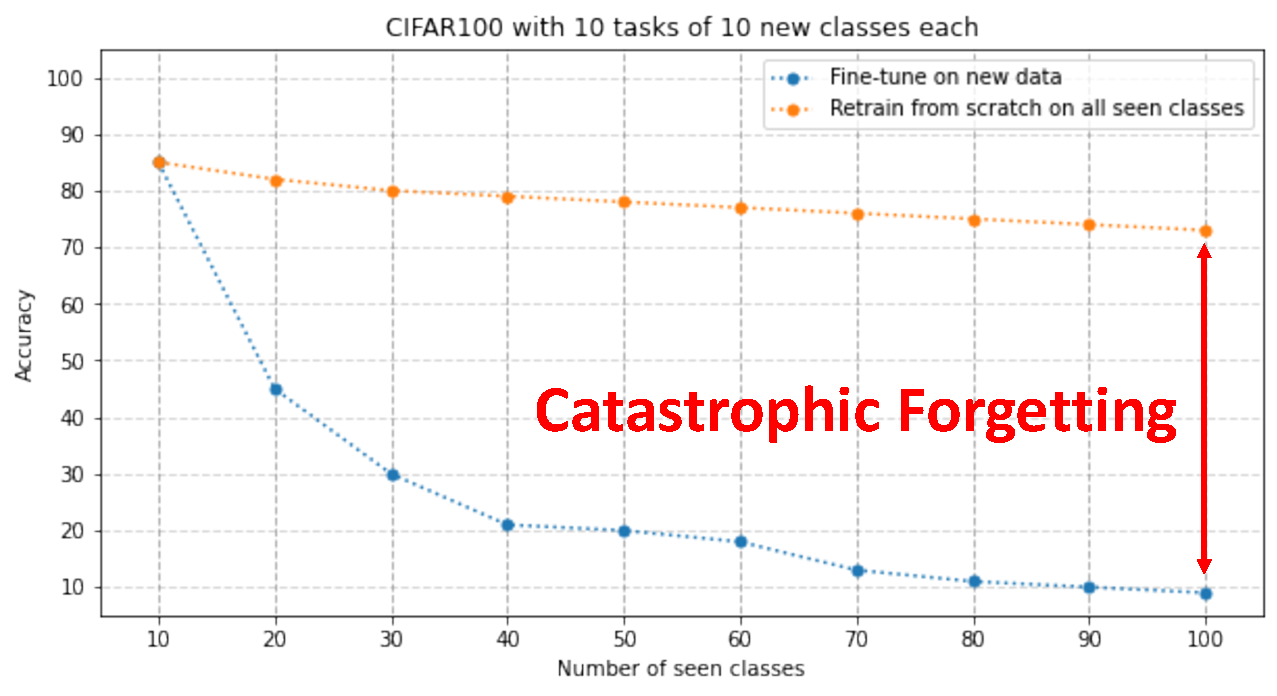
\includegraphics[width=0.8\linewidth]{images/related/catastrophic_forgetting.pdf}
    \end{center}
    \caption{\textbf{Training protocol for incremental learning}. At each training task we learn a
        new set of classes, and the model must retain knowledge about \textit{all} classes. The
        model is allowed a \textit{limited} memory of samples of old classes.}
    \label{fig:related_forgetting}
\end{figure}

\section{Rehearsal}

Multiple approaches exist to reduce catastrophic forgetting. The most efficient method is
\textbf{rehearsal learning} where old samples will be seen alongside the new samples. The amount of
old samples stored is extremely limited otherwise it would defect the purpose of continual learning.

Herding

Sampling

Pseudo-rehearsal

\begin{figure}[tb]
    \begin{center}
        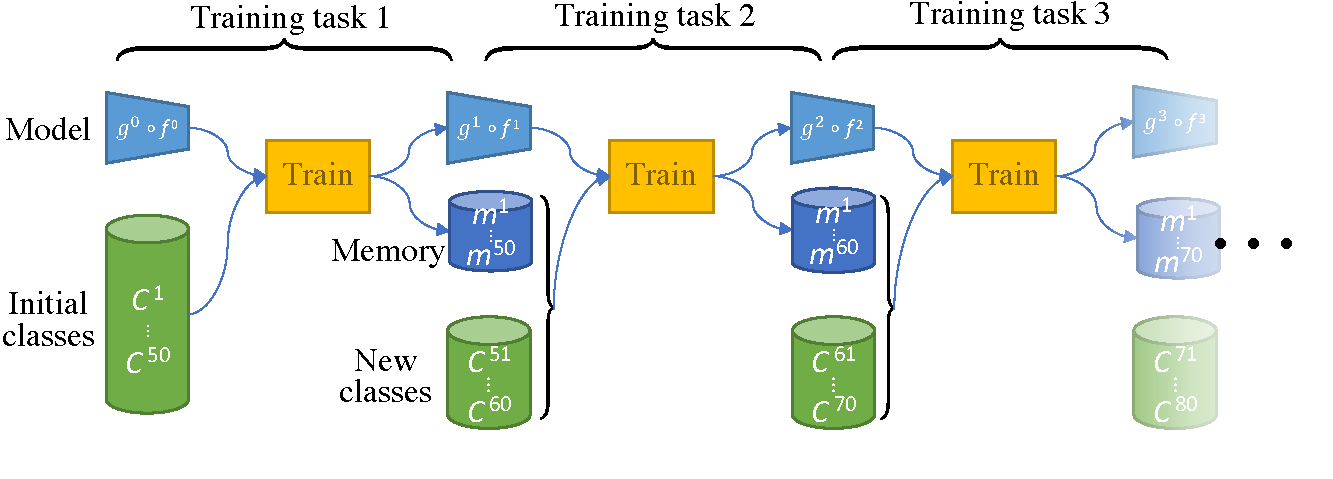
\includegraphics[width=0.8\linewidth]{images/podnet/protocol}
    \end{center}
    \caption{\textbf{Training protocol for incremental learning}. At each training task we learn a
        new set of classes, and the model must retain knowledge about \textit{all} classes. The
        model is allowed a \textit{limited} memory of samples of old classes.}
    \label{fig:related_protocol}
\end{figure}

\autoref{fig:related_protocol}


\section{Regularization-based Approaches}

\begin{figure}[tb]
    \begin{center}
        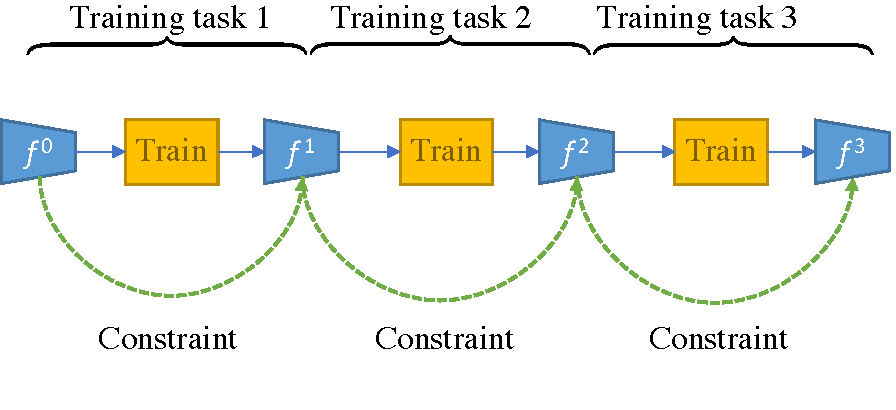
\includegraphics[width=0.8\linewidth]{images/related/continual_regularizations.pdf}
    \end{center}
    \caption{\textbf{Training protocol for incremental learning}. At each training task we learn a
        new set of classes, and the model must retain knowledge about \textit{all} classes. The
        model is allowed a \textit{limited} memory of samples of old classes.}
    \label{fig:related_regul}
\end{figure}

\subsection{Weight-based}

ewc, synaptic intelligence, riemmanian walk, memory aware synapses

however, \citep{lesort2019regulshortcomings} showed that


\subsection{Gradient-Based}

gem, agem, paper from aljundi with sampling

ogd, and the follow up paper with eigenvalues

\subsection{Output-based}

on probabilities: lwf, icarl, weight alignement

on embedding: ucir, mk2d

on attention maps: learning without memorizing

on intermediate statistics: paper from zagouraki, and pod and local pod

\section{Dynamic Strategies}

mask

growed networks

ensembing


\section{Optimization}

working on second order, flat minima

